%% The following is a directive for TeXShop to indicate the main file
%%!TEX root = diss.tex

\chapter{Preliminaries}
\label{ch:Preliminaries}

\begin{enumerate}
\item algebraic number theory background [edited once] \autoref{sec:AlgebraicNumberTheory}.
\item $p$-adics valuations [edited once] \autoref{sec:pAdicValuations}
\item $p$-adic logs \autoref{sec:pAdicLogarithms}
\item Setup with Lemmata from Samir
\item LLL [DONE - roughly]
\item Fincke-Pohst with changes from Benjamin [DONE- roughly]
\item linear forms in logs
\item Elliptic curves [DONE - rough]
\end{enumerate}

%---------------------------------------------------------------------------------------------------------------------------------------------%

\section{Algebraic number theory} 
\label{sec:AlgebraicNumberTheory}

\edit{Add some better intro: maybe see masters thesis}\\
\edit{In this section we recall some basic results from algebraic number theory that we use throughout the remaining chapters. We refer to \edit{Marcus} and \edit{Neukirch} for full details. Establish notation. The background for the material presented in this chapter is taken primarily from \edit{Marcus} and \edit{Neukirch}, and the material presented in \edit{}Section 2.2 can be found in [5]}

Let $K$ be a finite algebraic extension of $\mathbb{Q}$ of degree $n = [K:\mathbb{Q}]$. There are $n$ embeddings $\sigma: K \to \mathbb{C}$. These embeddings can be described by writing $K = \mathbb{Q}(\theta)$ for some $\theta \in \mathbb{C}$ and observing that $\theta$ can be sent to any one of its conjugates. 
Let $s$ denote the number of real embeddings of $K$ and let $t$ denote the number of conjugate pairs of complex embeddings of $K$, where $n = s + 2t$. By Dirichlet's Unit Theorem, the group of units of $K$ is the direct product of a finite cyclic group consisting of the roots of unity in $K$ and a free abelian group of rank $r = s + t -1$. Equivalently, there exists a system of $r$ independent units $\eps_1, \dots, \eps_r$ such that the group of units of $K$ is given by 
\[\left\{\zeta \cdot \eps_1^{a_1}\cdots \eps_r^{a_r} \ | \ \zeta \text{ a root of unity}, a_i \in \mathbb{Z} \text{ for } i = 1, \dots, r\right\}.\]
Any set of independent units that generate the torsion-free part of the unit group is called a system of \textit{fundamental units}. 

An element $\alpha \in K$ is called an \textit{algebraic integer} if its minimal polynomial over $\mathbb{Z}$ is monic. The set of algebraic integers in $K$ forms a ring, denoted $\mathcal{O}_K$. We refer to this ring as the \textit{ring of integers} or \textit{number ring} corresponding to the number field $K$. For any $\alpha \in K$, we define the \textit{norm} of $\alpha$ as 
\[N_{K/\mathbb{Q}}(\alpha) = \prod_{\sigma:K \to \mathbb{C}} \sigma(\alpha)\]
where the product is taken over all embeddings $\sigma$ of $K$. For algebraic integers, $N_{K/\mathbb{Q}}(\alpha) \in \mathbb{Z}$. The units are precisely the elements of norm $\pm 1$. Two elements $\alpha, \beta$ of $K$ are called \textit{associates} if there exists a unit $\eps$ such that $\alpha = \eps \beta$. Let $(\alpha)\mathcal{O}_K$ denote the ideal generated by $\alpha$. Associated elements generate the same ideal, and distinct generators of an ideal are associated. There exist only finitely many non-associated algebraic integers in $K$ with given norm. 

Any element of the ring of integers can be written as a product of \textit{irreducible} elements. These are non-zero non-unit elements of $\mathcal{O}_K$ which have no integral divisors but their own associates. Unfortunately, number rings are not alway unique factorization domains: this decomposition into irreducible elements may not be unique. However, every number ring is a Dedekind domain. This means that every ideal can be decomposed into a product of prime ideals and this decomposition is unique. A \textit{principal} ideal is an ideal generated by a single element $\alpha$. Two fractional ideals are called equivalent if their quotient is principal. It is well known that there are only finitely many equivalence classes of fractional ideals.  The number of classes is called the \textit{class number} of $\mathcal{O}_K$ and is denoted by $h_K$. For an ideal $\mathfrak{a}$, it is always true that $\mathfrak{a}^{h_K}$ is principal. The norm of the (integral) ideal $\mathfrak{a}$ is defined by $N_{K/\mathbb{Q}}(\mathfrak{a}) = \#\left(\mathcal{O}_K/\mathfrak{a}\right)$. If $\mathfrak{a} = (\alpha) \mathcal{O}_K$ is a principal ideal, then $N_{K/\mathbb{Q}}(\mathfrak{a}) = \left|N_{K/\mathbb{Q}}(\alpha)\right|$. 

Let $L$ be a finite field extension of $K$ with ring of integers $\mathcal{O}_L$. Every prime ideal $\mathfrak{P}$ of $\mathcal{O}_L$ \textit{lies over} a unique prime ideal $\mathfrak{p}$ in $\mathcal{O}_K$. That is, $\mathfrak{P}$ divides $\mathfrak{p}$. The \textit{ramification index} $e({\mathfrak{P}}|\mathfrak{p})$ is the largest power to which $\mathfrak{P}$ divides $\mathfrak{p}$. The field $\mathcal{O}_L/\mathfrak{P}$ is an extension of finite degree $f(\mathfrak{P}|\mathfrak{p})$ over $\mathcal{O}_K/\mathfrak{p}$. We call $f(\mathfrak{P}|\mathfrak{p})$ the \textit{inertial degree} of $\mathfrak{P}$ over $\mathfrak{p}$. For $\mathfrak{p}$ lying over the rational prime $p$, this is the integer such that 
\[N_{K/\mathbb{Q}}(\mathfrak{p}) = p^{f(\mathfrak{p}|p)}.\]
The ramification index and inertial degree are multiplicative in a tower of fields. In particular, if $\mathfrak{P}$ lies over $\mathfrak{p}$ which lies over the rational prime $p$, then
\[e({\mathfrak{P}}|p) = e({\mathfrak{P}}|\mathfrak{p})e({\mathfrak{p}}|p) \quad \text{ and } \quad f({\mathfrak{P}}|p) = f({\mathfrak{P}}|\mathfrak{p})f({\mathfrak{p}}|p).\]
Let $\mathfrak{P}_1, \dots, \mathfrak{P}_m$ be the primes of $\mathcal{O}_L$ lying over a prime ideal $\mathfrak{p}$ of $\mathcal{O}_K$. Denote by $e({\mathfrak{P}}_1|\mathfrak{p}),\dots, e({\mathfrak{P}}_m|\mathfrak{p})$ and $f({\mathfrak{P}}_1|\mathfrak{p}), \dots, f({\mathfrak{P}}_m|\mathfrak{p})$ the corresponding ramification indices and inertial degrees. Then
\[\sum_{i=1}^m e({\mathfrak{P}}_i|\mathfrak{p})f({\mathfrak{P}}_i|\mathfrak{p}) = [L:K].\]

If $L$ is normal over $K$ and $\mathfrak{P}_i$ and $\mathfrak{P}_j$ are two prime ideals lying over $\mathfrak{p}$, then $e({\mathfrak{P}}_i|\mathfrak{p}) = e({\mathfrak{P}}_j|\mathfrak{p})$ and $f({\mathfrak{P}}_i|\mathfrak{p}) = f({\mathfrak{P}}_j|\mathfrak{p})$. In this case, $\mathfrak{p}$ factors as
\[\mathfrak{p}\mathcal{O}_L = \left( \mathfrak{P}_1 \cdots \mathfrak{P}_m\right)^e\]
in $\mathcal{O}_L$, where the $\mathfrak{P}_i$ are distinct prime ideals all having the same ramification degree $e$ and inertial degree $f$ over $\mathfrak{p}$. It follows that 
\[mef = [L:K].\]

%---------------------------------------------------------------------------------------------------------------------------------------------%

\section{$p$-adic valuations}
\label{sec:pAdicValuations}

\edit{fix intro:
In this section we give a concise exposition of $p$-adic valuations. 
Everything in this document is based off of ``Elementary and analytic theory of algebraic numbers'' by W. Narkiewicz.
Throughout this thesis, we denote the algebraic closure of $\mathbb{Q}_p$ by $\overline{\mathbb{Q}}_p$. The completion of $\overline{\mathbb{Q}}_p$ with respect to the absolute value of $\overline{\mathbb{Q}}_p$ is denoted by $\mathbb{C}_p$.}

Let $K$ be an arbitrary number field. A homomorphism $v: K^* \to \mathbb{R}_{\geq 0}$ of the multiplicative group of $K$ into the group of positive real numbers is called a \textit{valuation} if it satisfies the condition
\[v(x+y) \leq v(x) + v(y).\]
This definition may be extended to all of $K$ by setting $v(0) = 0$. If
\[v(x+y) \leq \max(v(x),v(y))\]
holds for all $x,y \in K$, then $v$ is called a \textit{non-Archimedean valuation}. All remaining valuations on $K$ are called \textit{Archimedean}. 

Every valuation $v$ induces on $K$ the structure of a metric topological space which may or may not be complete. We say that two valuations are \textit{equivalent} if they define the same topology and we call an equivalence class of absolute values a \textit{place} of $K$. It is an elementary result of topology that every metric space may be embedded in a complete metric space, and this can be done in an essentially unique way. For the field $K$, the resulting complete metric space may be given a field structure. Equivalently, there exists a field $L$ with a valuation $w$ such that $L$ is complete in the topology induced by $w$. The field $K$ is contained in $L$ and the valuations $v$ and $w$ coincide in $K$. Moreover, the completion $L$ of $K$ is unique up to topological isomorphism.

For any non-zero prime ideal $\mathfrak{p}$ of $\mathcal{O}_K$, let $\ord_{\mathfrak{p}}(\mathfrak{a})$ denote the exact power to which $\mathfrak{p}$ divides the ideal $\mathfrak{a}$. For fractional ideals $\mathfrak{a}$ this number may be negative. For $\alpha \in K$, we write $\ord_{\mathfrak{p}}(\alpha)$ for $\ord_{\mathfrak{p}}\left((\alpha)\mathcal{O}_K\right)$. Every prime ideal defines a discrete non-Archimedean valuation on $K$ via
\[v(x):= \left(\frac{1}{N_{K/\mathbb{Q}}(\mathfrak{p})}\right)^{\ord_{\mathfrak{p}}(x)}.\]
Furthermore, every embedding of $K$ into the complex field defines an Archimedean valuation. Conversely, every discrete valuation on $K$ arises in this way by a prime ideal of $\mathcal{O}_K$, while every Archimedean valuation of $K$ is equivalent to $|\sigma(x)|$, where $\sigma$ is an embedding of $K$ into $\mathbb{C}$. Valuations defined by different prime ideals are non-equivalent, and two valuations defined by different embeddings of $K$ into $\mathbb{C}$ are equivalent if and only if those embeddings are complex conjugated. The topology induced in $K$ by a prime ideal $\mathfrak{p}$ of $\mathcal{O}_K$ is called the \textit{$\mathfrak{p}$-adic topology}. The completion of $K$ under this valuation is denoted by $K_{\mathfrak{p}}$ or $K_v$ and called the \textit{$\mathfrak{p}$-adic field}. Let $V$ be the set of all valuations of an algebraic number field $K$. Then for every non-zero element $\alpha \in K$ we have 
\[\prod_{v \in V} v(\alpha) = 1.\]

In the ring of integers of $\mathbb{Q}$, the prime ideals are generated by the rational primes $p$, and the resulting topology in the field $\mathbb{Q}$ is called the \textit{$p$-adic topology}. The completion of $\mathbb{Q}$ under this valuation is denoted by $\mathbb{Q}_p$. If $v(x)$ is a non-trivial valuation of $\mathbb{Q}$, then either $v(x)$ is equivalent to the ordinary absolute value $|x|$, or it is equivalent to one of the $p$-adic valuations induced by rational primes. Analogous to $\ord_{\mathfrak{p}}$, for any prime $p$ we define the $p$-adic order of $x \in \mathbb{Q}$ as the largest exponent of $p$ dividing $x$. Then, the $p$-adic valuation $v$ is defined as
\[v(x) = p^{-\ord_p(x)}.\]
If $K_{\mathfrak{p}}$ is a $\mathfrak{p}$-adic field, it is necessarily a finite extension of a certain $\mathbb{Q}_p$. 

Consider now $K/\mathbb{Q}$ where $n = [K:\mathbb{Q}]$ and let $g(t)$ denote the minimal polynomial of $K$ over $\mathbb{Q}$. Suppose $p$ is a rational prime and let $g(t) = g_1(t) \cdots g_m(t)$ be the decomposition of $g(t)$ into irreducible polynomials $g_i(t) \in \mathbb{Q}_p[t]$ of degree $n_i = \deg g_i(t)$. The prime ideals in $K$ dividing $p$ are in one-to-one correspondence with $g_1(t), \dots, g_m(t)$. More precisely, we have in $K$ the following decomposition of $(p)\mathcal{O}_K$
\[(p)\mathcal{O}_K = \mathfrak{p}_1^{e(\mathfrak{p}_1|p)} \cdots \mathfrak{p}_m^{e(\mathfrak{p}_m|p)},\]
with $\mathfrak{p}_1, \dots, \mathfrak{p}_m$ distinct prime ideals and ramification indices $e(\mathfrak{p}_1 | p), \dots, e(\mathfrak{p}_m | p) \in \mathbb{N}$. For $i = 1, \dots, m$ the inertial degree of $\mathfrak{p}_i$ is denoted by $f(\mathfrak{p}_i|p)$. Then $n_i = e(\mathfrak{p}_i | p)f(\mathfrak{p}_i | p)$ and $K_{\mathfrak{p}_i} \simeq \mathbb{Q}_p(\theta_i)$, where $g(\theta_i) = 0$. 

By $\overline{\mathbb{Q}_p}$ we denote the algebraic closure of $\mathbb{Q}_p$. There are $n$ embeddings of $K$ into $\overline{\mathbb{Q}_p}$, and each one fixes $\mathbb{Q}$ and maps $\theta$ to a root of $g$ in $\overline{\mathbb{Q}_p}$. Let $\theta_i^{(1)}, \dots, \theta_i^{(n_i)}$ denote the roots of $g_i(t)$ in $\overline{\mathbb{Q}_p}$. For $i = 1, \dots, m$ and $j = 1, \dots, n_i$, let $\sigma_{ij}$ be the embedding of $K$ into $\mathbb{Q}_p(\theta_i^{(j)})$ defined by $\theta \mapsto \theta_i^{(j)}$. The $m$ classes of conjugate embeddings are $\{\sigma_{i1}, \dots, \sigma_{in_i}\}$ for $i = 1, \dots, m$. Note that $\sigma_{ij}$ coincides with the embedding $K \hookrightarrow K_{\mathfrak{p}_i} \simeq \mathbb{Q}_p(\theta_i) \simeq \mathbb{Q}_p(\theta_i^{(j)})$. 

For any finite extension $L$ of $\mathbb{Q}_p$, the $p$-adic valuation $v$ of $\mathbb{Q}_p$ extends uniquely to $L$ as 
\[v(x) = |N_{L/\mathbb{Q}_p}(x)|^{1/[L:\mathbb{Q}_p]}.\]
Here, we define the $p$-adic order of $x \in L$ by
\[\ord_p(x) = \frac{1}{[L:\mathbb{Q}_p]}\ord_p(N_{L/\mathbb{Q}_p}(x)).\]
This definition is independent of the field $L$ containing $x$. So, since each element of $\overline{\mathbb{Q}_p}$ is by definition contained in some finite extension of $\mathbb{Q}_p$, this definition can be used to define the $p$-adic valuation $v$ of any $x \in \overline{\mathbb{Q}_p}$. Every finite extension of $\mathbb{Q}_p$ is complete with respect to $v$, but $\overline{\mathbb{Q}_p}$ is not. The completion of $\overline{\mathbb{Q}_p}$ with respect to $v$ is denoted by $\mathbb{C}_p$. 

The $m$ extensions of the $p$-adic valuation on $\mathbb{Q}$ to $K$ are just multiples of the $\mathfrak{p}_i$-adic valuation on $K$:
\[\ord_p(x) = \frac{1}{e_i}\ord_{\mathfrak{p}_i}(x) \quad \text{ for } i = 1, \dots, m.\]
We also view these extensions as arising from various embeddings of $K$ into $\overline{\mathbb{Q}_p}$. Indeed, the extension to $\mathbb{Q}_p(\theta_i^{(j)})$ of the $p$-adic valuation on $\mathbb{Q}_p$ induces a $p$-adic valuation on $K$ via the embedding $\sigma_{ij}$ as 
\[v(x) = |N_{K_{\mathfrak{p}_i}/\mathbb{Q}_p}(\sigma_{ij}(x))|^{1/n_i}.\]
Here, as before, $n_i = \deg g_i(t) = [K_{\mathfrak{p}_i} : \mathbb{Q}_p]$. Furthermore, 
\[\ord_p(x) = \ord_p(\sigma_{ij}(x)),\]
and we have
\[\ord_p(\sigma_{ij}(x)) =  \frac{1}{e_i}\ord_{\mathfrak{p}_i}(x) \quad \text{ for } i = 1, \dots, m,\ j = 1, \dots, n_i.\]

%---------------------------------------------------------------------------------------------------------------------------------------------%

\section{$p$-adic logarithms}
\label{sec:pAdicLogarithms}

Every non-zero $\alpha \in \mathbb{Q}_p$ has a $p$-adic expansion
\[\alpha = \sum_{i=k}^{\infty} u_ip^i\]
where $k = \ord_p(\alpha)$ and the $p$-adic digits $u_i$ are in $\{0, \dots, p-1\}$ with $u_k \neq 0$. If $\ord_p(\alpha) \geq 0$ then $\alpha$ is called a $p$-adic \textit{integer}. The set of $p$-adic integers is denoted $\mathbb{Z}_p$. A $p$-adic \textit{unit} is an $\alpha \in \mathbb{Q}_p$ with $\ord_p(\alpha) = 0$. For any $p$-adic integer $\alpha$ and $\mu \in \mathbb{N}_0$ there exists a unique rational integer $\alpha^{(\mu)} = \sum_{i=0}^{\mu-1}u_ip^i$ such that 
\[\ord_p(\alpha-\alpha^{(\mu)}) \geq \mu, \quad \text{ and } \quad 0 \leq \alpha^{(\mu)} \leq p^{\mu} - 1.\]
For $\ord_p(\alpha) \geq k$ we also write $\alpha \equiv 0 \mod{p^k}$. 

We have seen how to define $\ord_{\mathfrak{p}}$ and $\ord_p$ on algebraic extensions of $\mathbb{Q}$. For any $z \in \mathbb{C}_p$ with $\ord_p(z-1) > 0$, we can also define the $p$-adic logarithm of $z$ by
\[\log_p(z) = -\sum_{i=1}^{\infty} \frac{(1-z)^i}{i}.\]
By the $n^{\text{th}}$ term test, this series converges precisely in the region where $\ord_p(z-1) > 0$. Three important properties of the $p$-adic logarithm are
\begin{enumerate}
\item $\log_p(xy) = \log_p(x) + \log_p(y)$ whenever $\ord_p(x-1) > 0$ and $\ord_p(y-1) > 0$.
\item $\log_p(z^k) = k \log(p)$ whenever $\ord_p(z-1) > 0$ and $k \in \mathbb{Z}$. 
\item $\ord_p(\log_p(z)) = \ord_p(z-1)$ whenever $\ord_p(z-1) > 1/(p-1)$.
\end{enumerate}
\edit{where to find proofs?}

We shall use the following lemma to extend the definition of the $p$-adic logarithm to all $p$-adic units in $\overline{\mathbb{Q}_p}$. 
\begin{lemma} \label{Background:pAdicLemma}
Let $z$ be a $p$-adic unit belonging to a finite extensions $L$ of $\mathbb{Q}_p$. Let $e$ and $f$ be the ramification index and inertial degree of $L$. 
\begin{enumerate}
\item There is a positive integer $r$ such that $\ord_p(z^r-1) >0$.
\item If $r$ is the smallest positive integer having $\ord_p(z^r-1) >0$, then $r$ divides $p^f-1$, and an integer $q$ satisfies $\ord_p(z^q-1) >0$ if and only if it is a multiple of $r$.
\item If $r$ is a nonzero integer with $\ord_p(z^r-1) >0$, and if $k$ is an integer with $p^k(p-1) > e$, then
\[\ord_p(z^{rp^k}-1) >\frac{1}{p-1}.\]
\end{enumerate}
\end{lemma}
\edit{proofs?}

For $z$ a $p$-adic unit in $\overline{\mathbb{Q}_p}$ we define
\[\log_p{z} = \frac{1}{q}\log_p{z^q},\]
where $q$ is an arbitrary non-zero integer such that $\ord_p(z^q-1) >0$. To see that this definition is independent of $q$, let $r$ be the smallest positive integer with $\ord_p(z^r-1) >0$, and note that $q/r$ is an integer, and use the second property of $p$-adic logarithms above to write
\[\frac{1}{q}\log_p{z^q} = \frac{1}{r(q/r)}\log_p{z^{r(q/r)}} = \frac{1}{r}\log_p{z^r}.\]
Choosing $q$ such that $\ord_p(z^q-1) > 1/(p-1)$ helps to speed up and control the convergence of the series defining $\log_p$ \edit{refs}.

It is straightforward to see that Properties 1 and 2 above extend to the case where $x,y,z$ are $p$-adic units. Combining this with Property 3, we obtain
\begin{lemma}\label{Background:pAdicLemma2}
Let $z_1, \dots, z_m \in \overline{\mathbb{Q}_p}$ be $p$-adic units and let $b_1, \dots, b_m \in \mathbb{Z}$. If 
\[\ord_p(z_1^{b_1}\cdots z_m^{b_m} - 1) > \frac{1}{p-1}\]
then 
\[\ord_p(b_1\log_p{z_1} + \cdots + b_m \log_p{z_m}) = \ord_p(z_1^{b_1}\cdots z_m^{b_m} - 1).\]
\end{lemma}

%---------------------------------------------------------------------------------------------------------------------------------------------%



\section{The Weil height}
\label{sec:WeilHeight}

Let $k$ be a number field and at each place $v$ of $k$, let $k_v$ denote the completion of $k$ at $v$. Then
\[\sum_{v|p} [k_v:\mathbb{Q}_v] = [k:\mathbb{Q}]\]
for all places $p$ of $\mathbb{Q}$. We will use two normalized absolute values $| \ |_v$ and $\| \ \|_v$ on $k$ which we now define. If $v|\infty$, then $\| \ \|_v$ restricted to $\mathbb{Q}$ is the usual Archimedean absolute value; if $v|p$ for a rational prime $p$, then $\| \ \|_v$ restricted to $\mathbb{Q}$ is the usual $p$-adic absolute value. We then set
\[ | \ |_v = \| \ \|_v^{[k_v:\mathbb{Q}_v]/[k:\mathbb{Q}]}.\]
The \textit{logarithmic Weil height} $h: \overline{\mathbb{Q}} \to [0,\infty)$ is now defined as follows. Given $\alpha \in \overline{\mathbb{Q}}$, select any number field $k$ containing $\alpha$, and let 
\[h(\alpha) = \frac{1}{[k:\mathbb{Q}]}\sum_v \log^+|\alpha|_v,\]
the sum being taken over all places $v$ of $k$. The height does not depend on the choice of $k$ containing $\alpha$. We note that if $\alpha$ is an algebraic unit, then $|\alpha|_v = 1$ for all finite places $v$, and therefore $h(\alpha)$ can be taken over the infinite places only. 
In particular, if $\alpha \in \mathbb{Q}$, then with $\alpha = p/q$ for $p,q \in \mathbb{Z}$ with $\gcd(p,q) = 1$, we have $h(\alpha) = \log\max\{|p|,|q|\}$ and if $\alpha \in \mathbb{Z}$ then $h(\alpha) = \log|\alpha|$. \edit{check this}. 


%---------------------------------------------------------------------------------------------------------------------------------------------%
\subsection{Lattices: LLL and the Fincke-Pohst algorithm}
\edit{references for this are the two books living in the $x+y=z$ folder on the desktop}

\textbf{Lattices}
An $n$-dimensional lattice is a discrete subgroup of $\mathbb{R}^n$ of the form
\[\Gamma = \left\{ \sum_{i=1}^n x_i \mathbf{c}_i \ : \ x_i \in \mathbb{Z} \right\},\]
where $\mathbf{c}_1, \dots, \mathbf{c_n}$ are vectors forming a basis for $\mathbb{R}^n$. We say that the vectors $\mathbf{c}_1, \dots, \mathbf{c_n}$ form a \textit{basis} for $\Gamma$, or that they generate $\Gamma$. Let $B$ denote the matrix whose columns are the vectors $\mathbf{c}_1, \dots, \mathbf{c_n}$. Any lattice element $\mathbf{v}$ may be expressed as $\mathbf{v} = B\mathbf{x}$ for some $\mathbf{x} \in \mathbb{Z}^n$. 

A \textit{bilinear form} on a lattice $\Gamma$ is a function $\Phi: \Gamma \times \Gamma \to \mathbb{Z}$ satisying
\begin{enumerate}
\item $\Phi(\mathbf{u}, \mathbf{v}+\mathbf{w}) = \Phi(\mathbf{u},\mathbf{v}) + \Phi(\mathbf{u},\mathbf{w})$
\item $\Phi(\mathbf{u}+\mathbf{v}, \mathbf{w}) = \Phi(\mathbf{u},\mathbf{w}) + \Phi(\mathbf{v},\mathbf{w})$
\item $\Phi(a\mathbf{u}, \mathbf{w}) = a\Phi(\mathbf{u},\mathbf{w})$
\item $\Phi(\mathbf{u}, a\mathbf{w}) = a\Phi(\mathbf{u},\mathbf{w})$
\end{enumerate}
for all $\mathbf{u}, \mathbf{v}$, and $\mathbf{w}$ in $\Gamma$ and any $a \in \mathbb{R}$. 

In particular, given a basis we can define a specific bilinear form on our lattice $\Gamma$ as part of its structure. In the case of integral lattices, we have $\Phi: \Gamma \times \Gamma \to \mathbb{Z}$. This form describes a kind of distance between elements $\mathbf{x}$ and $\mathbf{y}$ of the lattice defined by $\Phi(\mathbf{x},\mathbf{y})$. 

A \textit{quadratic form} is a homogeneous polynomial of degree $2$. A form $Q$ is called positive definite if $Q(\mathbf{x})$ is strictly positive for any nonzero $\mathbf{x}$. A lattice is called \textit{positive definite} if its quadratic form is positive definite. 

A bilinear form has an associated quadratic form $Q: \Gamma \to \mathbb{Z}$ which is simply defined by $Q(\mathbf{x}) = \Phi(\mathbf{x}, \mathbf{x})$. The bilinear forms (and their associated quadratic forms) that we will be using come from the usual inner product on vectors in $\mathbb{R}^n$, also known as the dot product $\mathbf{u}\cdot \mathbf{v}$ for $\mathbf{u},\mathbf{v} \in \Gamma$, and multiplication with the basis matrix for coordinate vectors. That is, if $\mathbf{u} = B\mathbf{x}$ and $\mathbf{v} = B\mathbf{y}$ for a basis $B$, we have $\Phi(\mathbf{x},\mathbf{y}) = \mathbf{x}^TB^TB\mathbf{y}$. 

If $\mathbf{v} = B\mathbf{x}$, the \textit{norm} of the vector $\mathbf{v} \in \Gamma$ is defined by the quadratic form. We will be using the inner product $\mathbf{v} \cdot \mathbf{v}$. The norm of the coordinate vector $\mathbf{x}$ is then 
\[\mathbf{v}^T\mathbf{v} = (B\mathbf{x})^T(B\mathbf{x}) = \mathbf{x}^TB^TB\mathbf{x}.\]
Notice that this is also $\mathbf{x}^TA\mathbf{x}$ where $B^TB = A$. Here, $A$ is an example of the Gram matrix of $\Gamma$. The \textit{Gram matrix} of a lattice with basis $B$ with respect to a bilinear form $\Phi$ is defined to be the matrix A with entries $a_{ij} = \Phi(\mathbf{b}_i,\mathbf{b}_j)$.

The bilinear form on L can be written with respect to either embedded or coordinate vectors. Using another basis to express the lattice elements is possible, and sometimes preferable. But the Gram matrix is specific to the bilinear form on the lattice, and should not change when operating on embedded vectors. If it is operating on coordinate vectors, the change of basis must be accounted for.

If $A$ and $B$ are invertible $n \times n$ real matrices, then the lattice generated by the columns of $A$ is equal to the lattice generated by the columns of $B$ if and only if there is a unimodular matrix $U$ such that $AU = B$. 

\textbf{LLL}
\edit{Intro-ish: taken from Cohen p103
Among al1 the Z bases of a lattice L, some are better than others. The ones whose elements are the shortest (for the corresponding norm associated to the quadratic form q) are called reduced. Since the bases al1 have the same determinant, to be reduced implies also that a basis is not too far from being orthogonal.
The notion of reduced basis is quite old, and in fact in some sense one can even define an optimal notion of reduced basis. The problem with this is that no really satisfactory algorithm is known to find such a basis in a reasonable time, except in dimension 2 (Algorithm 1.3.14), and quite recently in dimension 3 from the work of B. Vall�e [Val].
A real breakthrough came in 1982when A. K. Lenstra, H. W. Lenstra and L. Lovkz succeeded in giving a new notion of reduction (what is now called
                                          2.6 Lattice Reduction Algorithms 85
     LLL-reduction) and simultaneously a reduction algorithm which is determin- istic and polynomial time (see [LLL]).This has proved invaluable.}

Let $\Gamma$ be a lattice with $\mathbf{c}_1, \dots, \mathbf{c}_n$. Define the vectors $\mathbf{c}_i^*$ for $i = 1, \dots, n$ and real numbers $\mu_{ij}$ ($1\leq j < i \leq n$) inductively by
\[\mathbf{c}_i^* = \mathbf{c}_i - \sum_{j=1}^{i-1}\mu_{ij}\mathbf{c}_j^*, \quad \mu_{ij} = \frac{\langle\mathbf{c}_i,\mathbf{c}_j^*\rangle}{\langle\mathbf{c}_j,\mathbf{c}_j^*\rangle}\]
(This is just the Gram-Scmidt process). The basis $\mathbb{c}_1,\dots, \mathbb{c}_n$ is called \textit{LLL-reduced} it
\[|\mu_{ij}| \leq \frac{1}{2} \quad \text{ for } 1\leq j < i \leq n, \]
\[\frac{3}{4}|\mathbb{c}_{i-1}^*|^2 \leq |\mathbb{c}_i^* + \mu_{ii-1}\mathbb{c}_{i-1}^*|^2 \quad \text{ for } 1 <i \leq n.\]

These properties implies that an LLL-reduced basis is approximately orthogonal, and that, generically, its constituent vectors are roughly of the same length. Every $n$-dimensional lattice has an LLL-reduced basis and such a basis can be computed very quickly using the so-called LLL algorithm (\edit{ref}). The LLL algorithm takes as input an arbitrary basis for a lattice and outputs an LLL-reduced basis for the lattice. The algorithm is typically modified to additionally output a unimodular matrix $U$ such that $B = AU$, where $A$ is the matrix whose column-vectors are the input basis and $B$ is the matrix whose column-vectors are the LLL-reduced output basis. Several versions of this algorirhm are implemented in MAGMA, including de Weger's exact integer version. (\edit{ref}).

For $\Gamma$ an $n$-dimensional lattice and $\mathbf{y}$ a vector in $\mathbb{R}^n$, we define
\[l(\Gamma,\mathbf{y}) = \min_{\mathbf{x} \in \Gamma \backslash\{\mathbf{y}\}} |\mathbf{x} - \mathbf{y}|.\]
The most important property of an LLL-reduced basis for us is the following lemma.
\begin{lemma}
\edit{lemma 18.1}
\end{lemma}
\edit{refs of where this lemma can be found - Cohen, for 1}
Note that the assumption in lemma \edit{cite} is equivalent to $\mathbf{y} \notin \Gamma$. 

\edit{Cohen:}  We see that the vector bl in a reduced basis is, in a very precise sense, not too far from being the shortest non-zero vector of L. In fact, it often is the shortest, and when it is not, one can, most of the time, work with bl instead of the actual shortest vector. As has already been mentioned, what makes al1these notions and theorems so valuable is that there is a very simple and efficient algorithm to find a reduced basis in a lattice. We now describe this algorithm in its simplest form.

\textbf{Fincke-Pohst}

We show how to modify the Fincke-Pohst algorithm to output short vectors in a translated lattice. That is, we compute the set of vectors $x$ such that 
\[(x-c)^tB^tB(x-c) \leq C\]
where $c$ is some vector over $\mathbb{Q}$ which represents the translation of our lattice. 


We begin with the usual Fincke-Pohst method for 
\[x^tB^tBx \leq C.\]
We call a vector $\mathbf{v}$ \textit{small} if its norm $\Phi(\mathbf{v}, \mathbf{v})$ is less than a constant $C$. This clearly depends on the basis which is given, and can vary depending on the choice of basis. If a particular basis is not specified, it is assumed to be the matrix $B$ which defines the Gram matrix $A = B^tB$. This is equivalent to solving the inequality $\Phi(\mathbf{y}, \mathbf{y}) \leq C$ where $\Phi(\mathbf{y}, \mathbf{y}) = \mathbf{y}^t\mathbf{y}$ denotes the norm of the vector computed with respect to the lattice. Let $B$ denote the matrix whose columns are the basis vectors of the lattice $\mathcal{L}$. As an element of the lattice, $\mathbf{y} = B\mathbf{x}$ for some coordinate vector $\mathbf{x} \in \mathbb{Z}^n$. So our inequality becomes
\[\Phi(\mathbf{y}, \mathbf{y}) = \mathbf{y}^t\mathbf{y} = \mathbf{x}^tB^tB\mathbf{x} \leq C.\] 
We consider the quadratic form $Q(\mathbf{x}) = \mathbf{x}^t B^t B\mathbf{x}$ and solve $Q(\mathbf{x}) \leq C$.

%---------------------------------------------------------------------------------------------------------------------------------------------%

\subsection*{Quadratic Completion}

To solve our inequality, it helps to first rearrange the terms of our quadratic form. This reformulation is called the quadratic completion or quadratic complementation. Here we assume the lattice is positive definite. That is, every nonzero element has a positive norm. With this, we can find the Cholesky decomposition $A = LL^t$, where $L$ is a lower triangular matrix. Equivalently, we can express this as $A = R^t R$, where $R$ is an upper triangular matrix. Since Fincke-Pohst uses upper triangular matrices, this is what we will use. The formulas below will reflect this. We now express $Q$ as:
\[ Q(\mathbf{x}) = \sum_{i=1}^m q_{ii}\left( x_i + \sum_{j=i+1}^m q_{ij}x_j\right)^2.\]

Our coefficients $q_{ij}$ are defined from $R$ and stored in a matrix for convenience.
\[q_{ij} =
\begin{cases}
\frac{r_{ij}}{r_{ii}} & \text{ if } i < j\\
r_{ii}^2 & \text{ if } i = j
\end{cases}.\]
Since $R$ is upper triangular, the matrix $Q = [q_{ij}]$ will be as well.

To obtain the upper triangular matrix $R$ from our matrix $A$, we compute the diagonal and non-diagonal entries as follows:
\[r_{ii} = \sqrt{ a_{ii} - \sum_{k = 1}^{i-1}r_{ki}^2}\]
\[r_{ij} = \frac{1}{r_{ii}}\left( a_{ij} - \sum_{k = 1}^{j-1}r_{ki}r_{kj}\right).\]

Using these, we can reformulate the construction of the coefficients of $Q$ to use values from $A$. We will soon see how it is possible to do away with using the Cholesky decomposition entirely.
\[q_{ii} = a_{ii} - \sum_{k = 1}^{i-1}r_{ki}^2\]
\[q_{ij} = \frac{1}{r_{ii}^2}\left( a_{ij} - \sum_{k = 1}^{j-1}r_{ki}r_{kj}\right).\]
By putting this construction in terms of the coefficients of Q only, we arrive at the following
\[q_{ii} = a_{ii} - \sum_{k = 1}^{i-1}q_{ki}^2q_{kk}\]
\[q_{ij} = \frac{1}{q_{ii}}\left( a_{ij} - \sum_{k = 1}^{j-1}q_{ki}q_{kj}q_{kk}\right).\]

We can then calculate these coefficients, starting with $q_{11}$ and calculating $q_{1j}$ for $1 \leq j \leq m$. Then we continue by calculating $q_{22}$ and $q_{2j}$ for $2 \leq j \leq m$. We proceed by first always calculating the diagonal entry $q_{ii}$ and then $q_{ij}$ for $i \leq j \leq m$ until we reach $q_{mm}$.
In practice, this is how we compute the coefficients for our form. However, it is equally possible to first compute the Cholesky Decomposition using available methods, and then computing the entries of $Q$ from this. In fact, we do exactly this, by first computing the Cholesky decomposition.

%---------------------------------------------------------------------------------------------------------------------------------------------%

\subsection*{The usual Fincke-Pohst way to bound $x_i$}

Since the sum $Q(x)$ is less than $C$, the individual term $q_{mm}x_m^2$ must also be less than $C$.
\begin{align*}
\sum_{i=1}^m q_{ii}\left( x_i + \sum_{j=i+1}^m q_{ij}x_j\right)^2	& \leq C \\
q_{mm}x_m^2 & \leq C\\\
x_m^2 & \leq \frac{C}{q_{mm}}.
\end{align*}
In fact, $x_m$ is bounded above by $\sqrt{C/q_{mm}}$ and below by $-\sqrt{C/q_{mm}}$. 

This illustrates the first step in establishing bounds on a specific entry $x_i$. Adding more terms from the outer sum to this sequence, a pattern emerges.
\begin{align*}
q_{mm}x_m^2 & \leq C\\
q_{m-1, m-1}\left(x_{m-1} + q_{m-1,m}x_m\right)^2 & \leq C - q_{mm}x_m^2\\
q_{m-2, m-2}\left(x_{m-2} + \sum_{j = m-1}^m q_{m-2,j}x_j\right)^2 & \leq C - q_{mm}x_m^2 - q_{m-1, m-1}\left(x_{m-1} + q_{m-1,m}x_m\right)^2\\
\end{align*}

Let
\[U_k = \sum_{j = k+1}^m q_{kj}x_j\]
so that we can rewrite $Q(\mathbf{x})$ as 
\[Q(\mathbf{x}) = \sum_{i=1}^m q_{ii}\left( x_i + \sum_{j=i+1}^m q_{ij}x_j\right)^2 = \sum_{i=1}^m q_{ii}\left( x_i + U_i\right)^2\]
In general, 
\[q_{kk}(x_k + U_k)^2 \leq C - \sum_{i = k+1}^m q_{ii}(x_i + U_i)^2.\]
Let $T_k$ denote the bound on the right-hand side. That is
\[T_k = C - \sum_{i = k+1}^m q_{ii}(x_i + U_i)^2,\]
so that $T_m = C$, $T_{m-1} = C - q_{mm}x_m^2$ and 
\[T_{m-2} = C - q_{mm}x_m^2 - q_{m-1, m-1}\left(x_{m-1} + q_{m-1,m}x_m\right)^2.\]

We set $T_m$ as $C$ and find each subsequent $T_k$ by subtracting the next term from the outer summand:
\[T_k = C - \sum_{i = k+1}^m q_{ii}(x_i + U_i)^2,\]
\[T_k = T_{k+1} - q_{k+1,k+1}(x_{k+1} + U_{k+1})^2.\]
Now, we have an upper bound for each summand. 
\[q_{kk}(x_k + U_k)^2 \leq T_k.\]
Using this, we can estimate upper and lower bounds for each $x_k$ in the coordinate vector $\mathbf{x}$. We start by computing the last entries of $\mathbf{x}$ and their bounds first. Assuming that the last several entries of $\mathbf{x}$ have been assigned, upper and lower bounds on $x_k$ can be determined. Now that we have established a bound on a term in the outer sum, we can determine bounds on the specific entry $x_k$. Take the above equation, and solve for $x_k$. Take the above equation and solve for $x_k$:
\begin{align*}
(x_k + U_k)^2	& \leq T_k/q_{kk}\\
	x_k + U_k	& \leq \sqrt{T_k/q_{kk}}\\
	x_k 		& \leq \sqrt{T_k/q_{kk}} - U_k.
\end{align*}
Similarly, we have a lower bound:
\[x_k \geq - \sqrt{T_k/q_{kk}} - U_k.\]
Since $x_k$ must be an integer, we can restrict our bounds further. Let $t_k = \sqrt{T_k/q_{kk}}$. 
\[UB_k = \lfloor t_k - U_k \rfloor\]
\[LB_k = \lceil-t_k - U_k\rceil\]
Here $UB_k$ is the upper bound on $x_k$ and $LB_k$ is the lower bound on $x_k$. 
\[LB_x \leq x_k \leq UB_k.\]

To enumerate all of the vectors $\mathbf{x}$ such that $Q(\mathbf{x}) \leq C$, begin with the last entry $x_m$ (letting all other $x_j = 0$). Determine the upper and lower bounds $UB_m$ and $LB_m$ by first calculating $t_m = \sqrt{T_m/q_{mm}}$. We define $U_m = 0$, and by definition remember that $T_m = C$.

For each entry $x_i$, starting with $x_m$ and going down to $x_1$, we initialize the value to be $x_i = LB_i$. After the value is initialized, we begin to increment the values of all the entries, adding 1 to each entry until we either reach the last index (in which case we have found a solution) or we exceed the upper bound on a particular entry (we will need to readjust the previously assigned entries). If at any time the lower bound exceeds the upper bound for a given entry, it will become immediately apparent when the value for that entry is initialized. We must then backtrack to our previous entries (that is, entries with a higher index). If we reach x1 without exceeding the upper bounds for any entry, then we have found a complete vector $\mathbf{x}$ which satisfies $Q(\mathbf{x}) \leq C$.

We will know we have found all the short vectors when we reach the zero vector. This is because we start by assigning each value $x_i$ its lower bound, which is calculated with respect to the values $x_{i+1}, \dots, x_n$. We increase $x_i$ incrementally, until it exceeds the corresponding calculated upper bound. When this happens we revisit $x_{i+1}$, increasing its value. Since $x_{i+1}$ was originally assigned its own lower bound, it starts off as a negative integer and increases steadily until it reaches $0$. Likewise, the other values will start off negative at each iteration and slowly increase in value. It is only when all entries are $0$ that the algorithm terminates. When we add each vector, we also add the vector with entries $-x_i$ for each $i$. In this we capture all the small vectors without having to check positive values for $x_n$.

Before beginning the search, first find the coefficients of the quadratic form expressed as above. Initialize $T_k,U_k,UB_k$ and $x_k$ to be $0$ for all $k$. Begin with $i = m$ and $T_i = C$ as the value bounding our vectors.

It is noted in the Fincke-Pohst paper that if we label the columns of $R$ by $\mathbf{r}_i$ (from the Cholesky decomposition $\mathbf{x}^tR^tR\mathbf{x}$) and the rows of $R^{-1}$ by $\mathbf{r}'_i$, then we see that 
\[x_i^2 = \left( \mathbf{r}'^t_i \left( \sum_{k=1}^m x_k \mathbf{r}_k\right) \right)^2 \leq \mathbf{r}'^t_i \mathbf{r}_i (\mathbf{x}^tR^tR\mathbf{x}) \leq \| \mathbf{r}'_i \|^2C.\]

So it may behoove us to reduce the rows of $R^{-1}$ in order to reduce our search space. Furthermore, it helps to put the smallest basis vectors first, so reordering the columns may also be beneficial.

Express this reduction with a unimodular matrix $V^{-1}$ so that $R_1^{-1} = V^{-1}R^{-1}$. Then reorder the columns of $R_1$ with a permutation matrix $P$. Since $R_1 = RV$, we then have that $R_2 = (RV)P$.

Then $R_2^{-1} = P^{-1}V^{-1}R^{-1}$. If we find a solution to the inequality $\mathbf{y}^tR_2^tR_2\mathbf{y}\leq C$, we can recover a solution to our original inequality by $\mathbf{x} = VP\mathbf{y}$. Since $R^{-1}_2 =P^{-1}V^{-1}R^{-1}$, we know that $R_2 = RVP$. 

\begin{align*}
\mathbf{y}^tR_2^tR_2\mathbf{y} & \leq C\\
\mathbf{y}^t(P^tV^tR^t)(RVP)\mathbf{y} & \leq C\\
(\mathbf{y}^tP^tV^t)R^tR(VP\mathbf{y}) & \leq C\\
(VP\mathbf{y})^tR^tR(VP\mathbf{y}) & \leq C\\
\mathbf{x}^tR^tR\mathbf{x} &\leq C.
\end{align*}

This improves the search time by giving us a nicer quadratic form to work with. Once we find solutions to the inequality given by $Q_2(\mathbf{y}) = \mathbf{y}^tR_2^tR_2\mathbf{y} \leq C$, it is a simple matter of translating them into solutions of our original inequality.

%---------------------------------------------------------------------------------------------------------------------------------------------%

\subsection{Translated Lattices}
We now explain how to apply Fincke-Pohst to the case
\[(x-c)^tB^tB(x-c) \leq C.\]
In place of the usual reduction listed above, we use MAGMA's built-in LLLGram function on the symmetric positive-definite matrix $A = B^tB$. Here, since $A$ is symmetric and positive-definite, it can be written as $A = R^tR$ for some upper triangular matrix $R$ (via Cholesky Decomposition).The function LLLGram, with input $A$, computes a matrix $G$ which is the Gram matrix corresponding to a LLL-reduced form of the matrix $R$. This function returns three values:
\begin{itemize}
\item A LLL-reduced Gram matrix $G$ of the Gram matrix $A$;
\item A unimodular matrix $U$ in the matrix ring over $\mathbb{Z}$ whose degree is the number of rows of $A$ such that $G=U^tAU$ (technically it returns $G=UAU^t$, but we change this here to simplify our computations later);
\item The rank of $A$ (which equals the dimension of the lattice generated by $R$).
\end{itemize}

Thus
\[(U^{-1})^tGU^{-1} = A\]
and we have
\begin{align*}
(x-c)^tB^tB(x-c) & \leq C\\
(x-c)^tA(x-c) & \leq C\\
(x-c)^t(U^{-1})^tGU^{-1}(x-c) \leq C\\
\left(U^{-1}(x-c)\right)^tG \left(U^{-1}(x-c)\right) \leq C\\
\left(y-d\right)^tG \left(y-d\right) \leq C
\end{align*}
where
\[y = U^{-1}x \quad \text{ and } \quad d = U^{-1}c.\]
Now, we are in position to enumerate the short vectors $y$ satisfying 
\[\left(y-d\right)^tG \left(y-d\right) \leq C.\]
We retrieve our solutions $x$ via $x = Uy$.

As before, we generate the matrix $Q$ such that 
\[ Q(\mathbf{x}) = \sum_{i=1}^m q_{ii}\left( y_i - d_i + \sum_{j=i+1}^m q_{ij}(y_j - d_j)\right)^2.\]

Since the sum $Q(x)$ is less than $C$, the individual term $q_{mm}(y_m - d_m)^2$ must also be less than $C$.
\begin{align*}
\sum_{i=1}^m q_{ii}\left( y_i - d_i + \sum_{j=i+1}^m q_{ij}(y_j - d_j)\right)^2	 & \leq C \\
q_{mm}(y_m - d_m)^2 & \leq C.
\end{align*}
Here, in place of the usual method of bounding $y_m - d_m$ by $\sqrt{C/q_{mm}}$ and $-\sqrt{C/q_{mm}}$, we instead let $y_m$ vary between $-\lfloor(-d_m)\rfloor$ and $-\lceil(-d_m)\rceil$. In this way, we simply need to verify that, for these choices of $y_m$, the equivalence
\[q_{mm}(y_m - d_m)^2 \leq C\]
is satisfied. If it is, we store this value of $y_m$, otherwise we let $y_m = y_m + 1$. This illustrates the first step in establishing bounds on a specific entry $y_i$. Adding more terms from the outer sum to this sequence, a pattern emerges.

Let
\[U_i = -d_i + \sum_{j = i+1}^m q_{ij}(y_j - d_j)\]
so that we can rewrite $Q(\mathbf{x})$ as 
\[ Q(\mathbf{x}) = \sum_{i=1}^m q_{ii}\left( y_i - d_i + \sum_{j=i+1}^m q_{ij}(y_j - d_j)\right)^2 = \sum_{i=1}^m q_{ii}\left( y_i + U_i\right)^2\]
In general, 
\[q_{kk}(y_k + U_k)^2 \leq C - \sum_{i = k+1}^m q_{ii}(y_i + U_i)^2.\]
Let $T_k$ denote the bound on the right-hand side. That is
\[T_k = C - \sum_{i = k+1}^m q_{ii}(y_i + U_i)^2,\]
so that $T_m = C$, $T_{m-1} = C - q_{mm}(y_m - d_m)^2$ and 
\[T_{m-2} = C - q_{mm}(y_m - d_m)^2 - q_{m-1, m-1}\left(y_{m-1} - d_{m-1} + q_{m-1,m}(y_m-d_m)\right)^2.\]

We set $T_m$ as $C$ and find each subsequent $T_k$ by subtracting the next term from the outer summand:
\[T_k = C - \sum_{i = k+1}^m q_{ii}(y_i + U_i)^2,\]
\[T_k = T_{k+1} - q_{k+1,k+1}(y_{k+1} + U_{k+1})^2.\]
Now, we have an upper bound for each summand. 
\[q_{kk}(y_k + U_k)^2 \leq T_k.\]
Using this, we can estimate upper and lower bounds for each $y_k$ in the coordinate vector $\mathbf{y}$. We start by computing the last entries of $\mathbf{y}$ and their bounds first. Assuming that the last several entries of $\mathbf{y}$ have been assigned, upper and lower bounds on $y_k$ can be determined. Now that we have established a bound on a term in the outer sum, we can determine bounds on the specific entry $y_k$. The following diagram illustrates the scenario. In the usual Fincke-Pohst algorithm, we take the above equation and solve for $y_k$:
\begin{align*}
(y_k + U_k)^2	& \leq T_k/q_{kk}\\
	y_k + U_k	& \leq \sqrt{T_k/q_{kk}}\\
	y_k 		& \leq \sqrt{T_k/q_{kk}} - U_k.
\end{align*}
Similarly, we have a lower bound:
\[y_k \geq - \sqrt{T_k/q_{kk}} - U_k.\]
Since $x_k$ must be an integer, we can restrict our bounds further. Let $t_k = \sqrt{T_k/q_{kk}}$. 
\[UB_k = \lfloor t_k - U_k \rfloor\]
\[LB_k = \lceil-t_k - U_k\rceil\]
Here $UB_k$ is the upper bound on $y_k$ and $LB_k$ is the lower bound on $y_k$. 
\[LB_k \leq y_k \leq UB_k.\]

\subsection{Refinements}
We note here that computing $LB_k$ and $UB_k$ is highly inefficient as it often requires high precision to accurately compute $\sqrt{T_k/q_{kk}}$. Instead, we adopt the following bounds, as per Matshke's algorithm. To help justify this process, we refer to the following diagram

\begin{center}
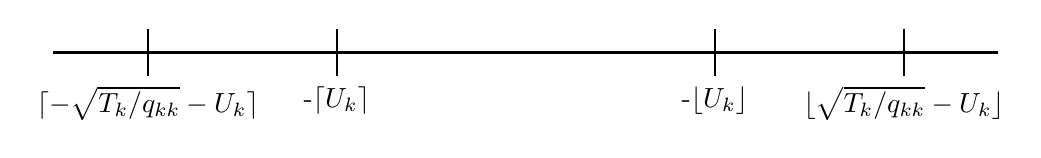
\begin{tikzpicture}[scale=6]
\draw[thick] (0.8,0.05)--(0.8,-0.05) node[anchor=north] {$\lfloor \sqrt{T_k/q_{kk}} - U_k \rfloor$};
\draw[thick] (-0.8,0.05)--(-0.8,-0.05) node[anchor=north]{$\lceil -\sqrt{T_k/q_{kk}} - U_k \rceil$};
\draw[thick] (0.4,0.05)--(0.4,-0.05) node[anchor=north] {-$\lfloor U_k \rfloor$};
\draw[thick] (-0.4,0.05)--(-0.4,-0.05) node[anchor=north]{-$\lceil U_k \rceil$};
\draw[thick] (-1,0)--(1,0);
\end{tikzpicture}
\end{center}

As stated above, 
\[\lceil -\sqrt{T_k/q_{kk}} - U_k \rceil= LB_k \leq y_k \leq UB_k = \lfloor \sqrt{T_k/q_{kk}} - U_k \rfloor.\]
In our old implementation for non-translated lattices, we set each $y_k = LB_k$ and increased each term until we reached the zero (centre) vector. Here since the centre vector is non-zero, we instead set each $y_k = -\lceil U_k \rceil$ and increase each $y_k$ successively until $y_k > \lfloor \sqrt{T_k/q_{kk}} - U_k \rfloor$. This is equivalent to the above computation and generates only half of the vectors, assuming symmetry. This symmetry can only be applied if the centre vector is defined over $\mathbb{Z}$, otherwise we must compute all vectors. To do (we can also break symmetry and compute all vectors in the $\mathbb{Z}$ case), we also set $y_k = \lceil U_k \rceil - 1$ and successively decrease this term until $y_k <\lceil -\sqrt{T_k/q_{kk}} - U_k \rceil$.

Of course, in this refinement, we want to avoid computing $\sqrt{T_k/q_{kk}}$, and so instead of verifying whether $y_k > \lfloor \sqrt{T_k/q_{kk}} - U_k \rfloor$ or $y_k <\lceil -\sqrt{T_k/q_{kk}} - U_k \rceil$, we compute $q_{kk}(y_k + U_k)^2$ in each case and verify whether
\[q_{kk}(y_k + U_k)^2 \leq C - \sum_{i = k+1}^m q_{ii}(y_i + U_i)^2\]
holds. In the first round, if this does not hold and if $y_k < -\lfloor U_k \rfloor$, we continue to iterate $y_k = y_k + 1$, otherwise we simply iterate $y_k = y_k + 1$. Once this equivalence does not hold and $y_k \geq -\lfloor U_k \rfloor$, we stop this loop. We then reset $y_k = \lceil U_k \rceil - 1$ and search in the other direction, by successively subtracting $1$ if 
\[q_{kk}(y_k + U_k)^2 \leq C - \sum_{i = k+1}^m q_{ii}(y_i + U_i)^2\]
holds. We stop searching in this direction only once this equivalence does not hold.  

%---------------------------------------------------------------------------------------------------------------------------------------------%

\subsection{Preliminaries: Elliptic Curves}

Let $K$ be a field. An \textit{elliptic curve} $E$ over $K$ is a nonsingular curve of the form 
\begin{equation} \label{elliptic}
E: y^2 + a_1xy + a_3y = x^3 + a_2x^2 + a_4x + a_6
\end{equation}
with $a_i \in K$, having a specified base point, $\mathcal{O}\in E$. An equation of the form (\ref{elliptic}) is called a \textit{Weierstrass equation}. For an elliptic curve $E$ over $K$, this equation is unique up to a coordinate transformation of the form
\[x = u^2x' + r, \quad\quad y = u^3y' + su^2x' + t, \]
with $r,s,t,u \in K, u\neq 0$. 
Writing 
\[b_2 = a_1^2 + 4a_2, \quad b_4 = a_1a_3 + 2a_4, \quad b_6 = a_3^2 + 4a_6,\]
\[b_8 = a_1^2a_6 + 4a_2a_6 - a_1a_3a_4 + a_2a_3^2 - a_4^2,\]
\[ c_4 = b_2^2 - 24b_4, \quad \text{ and } \quad c_6 = -b_2^3 + 36b_2b_4 + 9b_2b_4b_6,\]
if $\text{char}(K) \neq 2,3$, we can make several linear changes of variables so that, using these values, our elliptic curve has equation
\begin{equation} \label{curve}
E: y^2 = x^3 - 27c_4x - 54c_6.
\end{equation}
Associated to this curve are the quantities 
\[\Delta = -b_2^2b_8 - 8b_4^3 - 27b_6^2 + 9b_2b_4b_6 \quad \text{ and } \quad j = c_4^3/\Delta,\]
where $\Delta$ is called the \textit{discriminant} of the Weierstrass equation, and the quantity $j$ is called the \textit{j-invariant} of the elliptic curve. The condition of being nonsingular is equivalent to $\Delta$ being non-zero. Additionally, one may show that two elliptic curves are isomorphic over $\bar{K}$, the algebraic closure of $K$, if and only if they both have the same $j$-invariant.

When $K = \mathbb{Q}$, we can choose the Weierstrass model (\ref{elliptic}) with the $a_i \in \mathbb{Z}$ and the $p$-order of $\Delta$ minimal for each prime $p$. Supposing (\ref{elliptic}) is such a global minimal model for an elliptic curve $E$ over $\mathbb{Q}$, reducing the coefficients modulo a prime $p$, we obtain a (possibly singular) curve over $\mathbb{F}_p$, namely
\begin{equation}
\tilde{E}: y^2 + \tilde{a_1}xy + \tilde{a_3}y = x^3 + \tilde{a_2}x^2 + \tilde{a_4}x + \tilde{a_6},
\end{equation}
with $\tilde{a_i} \in \mathbb{F}_p$. This ``reduced" curve $\tilde{E}/\mathbb{F}_p$ is called the \textit{reduction of $E$ modulo} $p$. It is nonsingular provided that $\Delta \not \equiv 0 \mod{p}$, in which case it is an elliptic curve defined over $\mathbb{F}_p$. The curve $E$ is said to have \textit{good reduction} modulo $p$ if $\tilde{E}/\mathbb{F}_p$ is nonsingular, otherwise, we say $E$ has \textit{bad reduction} modulo $p$. 

The bad reduction of $E$ is measured by the \textit{conductor} of $E$, 
\[N = \prod_{p \text{ prime }}p^{f_p}, \]
where $f_p \neq 0$ if $p \nmid \Delta$ (so $f_p = 0$ for all but finitely many primes $p$), while $f_p = 1$ if the singularity is a node, and $f_p \geq 2$ if the singularity is a cusp. The $f_p$, hence the conductor, are invariant under isogeny. Hence, roughly speaking, the conductor $N$ is the product of primes at which $E$ has bad reduction raised to small powers, while the discriminant $\Delta$ is a product of the same primes, but they may sometimes appear to large powers.

%-----------------------------------------------------------------------------------------------------------------------------------------------
\subsection{Preliminaries: Cubic Forms}

Let $a,b,c$ and $d$ be integers, and consider the binary cubic form
\[F(x,y) = ax^3 + bx^2y + cxy^2 + dy^3.\]
Two such forms $F_1$ and $F_2$ are called \textit{equivalent} if they are equivalent under the $GL_{2}(\mathbb{Z})$-action. That is, if there exist integers $a_1, a_2, a_3$, and $a_4$ such that 
\[F_1(a_1x + a_2y, a_3x + a_4y) = F_2(x,y)\]
for all $x,y$, where $a_1a_4 - a_2a_3 = \pm 1$. In this case, we write $F_1 \sim F_2$. The \textit{discriminant} $D_F$ of such a form is given by 
\[D_F = -27a^2d^2 + b^2c^2 + 18abcd - 4ac^3 - 4b^3d = a^4 \prod_{i < j} (\alpha_i - \alpha_j)^2\]
where $\alpha_1, \alpha_2$ and $\alpha_3$ are the roots of the polynomial $F(x,1)$. We observe that if $F_1 \sim F_2$, then $D_{F_1} = D_{F_2}$. 

Associated to $F$ is the Hessian $H_F(x,y)$, given by
\begin{align*}
H_F(x,y) & = -\frac{1}{4}\left( \frac{\partial^2F}{\partial x^2} \frac{\partial^2F}{\partial y^2} - \left(\frac{\partial^2F}{\partial x \partial y}\right)^2\right)\\
& = (b^2 - 3ac)x^2 + (bc - 9ad)xy + (c^2 - 3bd)y^2,
\end{align*}
and the Jacobian determinant of $F$ and $H$, a cubic form $G_F(x,y)$ defined via 
\begin{align*}
G_F(x,y) &= \frac{\partial F}{\partial x} \frac{\partial H}{\partial y} - \frac{\partial F}{\partial y} \frac{\partial H}{\partial x} \\
& =  (-27a^2d + 9abc -2b^3)x^3 + (-3b^2c - 27abd + 18ac^2)x^2y +  \\
& \quad \quad + (3bc^2 - 18b^2d + 27acd)xy^2 + (-9bcd + 2c^3 + 27ad^2)y^3.
\end{align*}





\endinput

Any text after an \endinput is ignored.
You could put scraps here or things in progress.